%===============================================================================


%===============================================================================
%\documentclass[usenatbib, usegraphicx]{mnras}
\documentclass[usenatbib]{mnras}

\usepackage{graphicx}
\usepackage{hyperref}
\usepackage{xspace}
\usepackage{amsmath}

%\newcommand{\boldsymbol}[1]{\mbox{\boldmath{${#1}$}}}

\def\psio{\psi(0)}
\def\psii{\psi'}
\def\psiii{\psi''}
\def\psiiii{\psi'''}
\def\psiiiisq{\psi'''^{2}}
\def\psiiv{\psi^{(iv)}}

\def\psicomb{\tilde{\psi}'''}
\def\radmagrat{r_{\mu_r}}

\def\tein{\theta_{\mathrm{E}}}
\def\reff{R_e}
\def\sigmae{\sigma_{e2}}
\def\mdme{M_{\mathrm{DM},e}}
\def\gammadm{\gamma_{\mathrm{DM}}}

\def\hyperp{\boldsymbol{\eta}}
\def\individ{\boldsymbol{\psi}}
\def\individi{\boldsymbol{\psi}_i}
\def\individsamp{\boldsymbol{\psi}_{i}^{(k)}}
\def\data{\mathbf{d}}
\def\datai{\mathbf{d}_i}
\def\wl{\left\{\rm{WL}\right\}}

\def\Sref#1{Section~\ref{#1}\xspace}
\def\Fref#1{Figure~\ref{#1}\xspace}
\def\Tref#1{Table~\ref{#1}\xspace}
\def\Eref#1{Equation~\ref{#1}\xspace}

\def\pr{{\rm P}}

%===============================================================================

\begin{document}

\title{On power-law profiles in time delay cosmography}
\author[Sonnenfeld \& Marshall]{
Alessandro~Sonnenfeld,$^{1}$\thanks{E-mail:alessandro.sonnenfeld@ipmu.jp}
Philip~J.~Marshall,$^{2}$
\\
$^{1}$Kavli IPMU (WPI), UTIAS, The University of Tokyo, Kashiwa, Chiba 277-8583, Japan \\
%$^{1}$Kavli Institute for the Physics and Mathematics of the Universe (WPI),The University of Tokyo Institutes for Advanced Study, The University of Tokyo, Kashiwa, Chiba 277-8583, Japan \\
$^{2}$ Kavli Institute for Particle Astrophysics and Cosmology, Stanford University, 452 Lomita Mall, Stanford, CA 94035, USA\\
}

\maketitle

%-------------------------------------------------------------------------------
\begin{abstract}
Time-delay lensing is a mature and competitive cosmological probe.
However, it suffers from the well-known problem of the mass-sheet degeneracy:
too rigid assumptions on the density profile of the lens can bias the inference on the Hubble constant.
We investigate in detail the degeneracy between the choice of the lens density profile and the inference on cosmology, focusing on double systems.
By expanding lensing observables in terms of the local derivatives of the lens potential around the Einstein radius, in the case of circular lenses,
we show that three degrees of freedom in the radial direction are necessary to achieve a few percent accuracy in the time-delay distance, even in cases where the asymmetry in the image configuration is relatively small.
We also show that, while the time delay is strongly dependent on the second derivative of the potential, observables typically used to constrain lens models in time-delay studies, such as image position and radial magnification information, are mostly sensitive to the first and third derivatives, making it very challenging to accurately determine time-delay distances with lensing data alone.
We generate an ensemble of mock observations and show that the assumption of a power-law density profile results in a 10\% bias on $H_0$.
Using a more flexible model and adding velocity dispersion constraints allows, under optimistic assumptions on the dynamical modeling, to obtain an inference with 1\% accuracy.
Although all of our treatment is based on the assumption of axisymmetry, our findings can be generalized to cases with moderate ellipticity.
\end{abstract}

\begin{keywords}
   galaxies: elliptical and lenticular, cD -- galaxies: evolution
\end{keywords}

%-------------------------------------------------------------------------------
\section{Introduction}\label{sect:intro}

One of the obstacles in time delay lens cosmography is set by the mass sheet degenerac.
\citet{S+S13} showed that the assumption of a power-law density profile can introduce a large bias in the inferred value of the Hubble constant, in cases when the true density profile is not a pure power-law.
Here we investigate further this issue.

We wish to determine what is the minimum number of degrees of freedom in the lens density profile in order to reproduce lensing observables and time delays within a given accuracy goal.
We limit our study to double image systems. Furthermore, we assume circular symmetry throughout our work. Most of the results derived here can be generalized to the non-axisymmetric case.

\section{Lensing observables and lens potential derivatives}\label{sect:pot}

Let us consider a circularly symmetric lens with Einstein radius $\tein$.
Let $\beta$ and $\theta$ be angular coordinates in the source and image plane respectively, with origin at the optical axis and same orientation.
Let $\psi(\theta)$ denote the lens potential.
We wish to determine which aspects of $\psi(\theta)$ are different lensing observables sensitive to.
This has been done in the general, non-asisymmetric case, by \cite{W+B16}, by expanding the lens potential around the center of the lens.
Here we adopt a similar approach, but focus on derivatives of the potential around the Einstein radius.

Let us consider a source at position $\beta_s>0$, lying within the radial caustic.
The corresponding image positions are determined by the lens equation:
\begin{equation}
\beta_s = \theta  - \alpha(\theta).
\end{equation}
For non-singular lenses, three images will form: one at $\theta_A > \tein$, and the other two at $-\tein < \theta_B < \theta_C < 0$.
The image at $\theta_C$ is, usually, highly demagnified, and we will ignore it from now on.
For small values of $\beta_s$, images A and B will be close to the critical curve. We can then do a Taylor expansion of the lens equation around $\theta=\tein$.
The lens potential at a position $\theta_A = \tein + \Delta\theta_A$ is, to third order in $\Delta\theta_A$,
\begin{equation}\label{eq:potA}
\psi(\theta_A) = \psio + \psii \Delta\theta_A + \frac12 \psiii \Delta\theta_A^2 + \frac16 \psiiii \Delta\theta_A ^ 3,
\end{equation}
where $\psio$ is the (arbitrary) value of the potential at the Einstein radius, $\psi(\tein)$, and $\psii$, $\psiii$, $\psiiii$ are the first, second and third derivatives of the potential evaluated at the Einstein radius:
\begin{equation}
\psii \equiv \left. \frac{d\psi}{d\theta} \right\rvert_{\theta=\tein},
\end{equation}
\begin{equation}
\psiii \equiv \left. \frac{d^2\psi}{d\theta^2} \right\rvert_{\theta=\tein},
\end{equation}
\begin{equation}
\psiiii \equiv \left. \frac{d^3\psi}{d\theta^3} \right\rvert_{\theta=\tein}.
\end{equation}
The first derivative of the lens potential is the deflection angle $\alpha(\theta)$, which, evaluated at the Einstein radius, is equal to the Einstein radius:
\begin{equation}\label{eq:rein}
\psii = \tein.
\end{equation}
Similarly to \Eref{eq:potA}, the potential at a position $\theta_B = -\tein + \Delta\theta_B$ is, to third order in $\Delta\theta_B^3$,
\begin{equation}\label{eq:potB}
\psi(\theta_B) = \psio - \psii \Delta\theta_A + \frac12 \psiii \Delta\theta_A^2 - \frac16 \psiiii \Delta\theta_A ^ 3,
\end{equation}
where we have used the symmetry of the lens potential around $\theta = 0$.
The lens equation for image A reads
\begin{equation}
\beta_s = \theta_A - \psii - \psiii \Delta\theta_A - \frac12 \psiiii \Delta\theta_A^2.
\end{equation}
Using $\theta_A = \tein + \Delta\theta_A$ and \Eref{eq:rein}, this simplifies to
\begin{equation}\label{eq:imA}
\beta_s = \Delta\theta_A - \psiii \Delta\theta_A - \frac12 \psiiii \Delta\theta_A^2.
\end{equation}
For image B, the same procedure leads to
\begin{equation}\label{eq:imB}
\beta_s = \Delta\theta_B - \psiii \Delta\theta_B + \frac12 \psiiii \Delta\theta_A^2.
\end{equation}
By equating the right hand sides of \Eref{eq:imA} and \Eref{eq:imB}, we obtain a second order equation in $\Delta\theta_A$ and $\Delta\theta_B$.
Solving for $\Delta\theta_B$, we obtain
\begin{equation}
\Delta\theta_B = \frac{1-\psiii}{\psiiii}\left[-1 + \sqrt{1 - 2(1-\psiii)\psiiii - \psiiiisq\Delta\theta_A^2}\right].
\end{equation}
Taylor expansion of the above equation to second order in $\Delta\theta_A$ gives
\begin{equation}\label{eq:lens2nd}
\Delta\theta_B = \Delta\theta_A - \frac{\psiiii}{1-\psiii}\Delta\theta_A^2 + O(\max{\{\Delta\theta_A^3, \Delta\theta_B^3\}}).
\end{equation}
%
\Eref{eq:lens2nd} relates the position of image B to that of image A and the derivatives of the potential.
The dependence of the Einstein radius is implicit in the definition of $\Delta\theta_A$ and $\Delta\theta_B$.

Let us now examine how different observables depend on the lens potential derivatives.
Let us start with the image separation. To second order in $\Delta\theta_A$, this reads
\begin{equation}\label{eq:imsep}
\theta_A - \theta_B = 2\psii + \frac{\psiiii}{1-\psiii}\Delta\theta_A^2,
\end{equation}
that is, the image separation is approximately equal to twice the Einstein radius.

Let us now consider the magnification. Absolute magnification is only observable if the lensed source is a standard candle, or a standard ruler.
The ratio of magnifications of different images of the same source is more easily accessible. Still, in the case of lensed quasars, the magnification ratio due to the main lens is difficult to measure accurately, due to microlensing or the presence of substructure.
Nevertheless, some constraints on magnification can be obtained by careful modeling of the images of a lensed extended source.
In detailed time delay lens studies, for instance, the slope of the density profile of the lens is usually constrained by fitting a parametrized model to the full surface brightness distribution of the quasar host galaxy. %a lensed extended source,
%which in the case of lensed quasars is usually the quasar host galaxy.
%Nevertheless, when detailed lens modeling is performed, in which the full surface brightness distribution of a lensed extended source is reproduced, some constraints on magnification can be obtained.
This constraint from extended source modeling is essentially a measurement of radial magnification ratio. 
When an extended source is lensed into two arcs at two different distances from the lens, the ratio between the arc widths, which is directly observable, is given by the ratio of radial magnifications at the two positions.

Radial magnification, for a circular lens, is defined as
\begin{equation}
\mu_r = \left(\frac{d\beta}{d\theta}\right)^{-1} = \left(1 - \frac{d\alpha}{d\theta}\right)^{-1}.
\end{equation}
The Taylor expansion around image A of the second derivative of the deflection angle is,
\begin{equation}
\frac{d\alpha(\theta_A)}{d\theta} = \psiii + \psiiii\Delta\theta_A + \psiiv\Delta\theta_A^2 + O(\Delta\theta_A^3).
\end{equation}
For image B,
\begin{equation}
\frac{d\alpha(\theta_A)}{d\theta} = \psiii - \psiiii\Delta\theta_A + \psiiv\Delta\theta_A^2 + O(\Delta\theta_B^3).
\end{equation}
Radial magnification introduces the fourth order derivative of the potential. This, however, cancels out when taking the ratio between the magnifications at image A and B. The result is the following:
\begin{equation}\label{eq:radmagrat}
\frac{\mu_{r,A}}{\mu_{r,B}} = 1 + \frac{2\psiiii}{1-\psiii}\Delta\theta_A + \left(\frac{\psiiii}{1-\psiii}\right)^2\Delta\theta_A^2 + O(\Delta\theta^3).
\end{equation}

Finally, we consider the time delay between image A and B. This is given by
\begin{equation}\label{eq:dt}
\Delta t = \frac{D_{\Delta t}}{c}\left[\frac{(\theta_A - \beta_s)^2}{2} - \psi(\theta_A) - \frac{(\theta_B - \beta_s)^2}{2} + \psi(\theta_B)\right],
\end{equation}
where $c$ is the speed of light, and $D_{\Delta t}$ is the so-called time-delay distance. This, in turn, is defined as
\begin{equation}
D_{\Delta t} \equiv (1+z_d) \frac{D_d D_s}{D_{ds}},
\end{equation}
where $z_d$ is the redshift of the lens, $D_d$, $D_s$ are the angular diameter distances of the lens and source relative to the observer, and $D_{ds}$ the angular diameter distance between lens and source. 

Substituting Equations \ref{eq:potA}, \ref{eq:potB}, \ref{eq:imA}, \ref{eq:imB} and \ref{eq:lens2nd} into \Eref{eq:dt}, and keeping terms up to second order in $\Delta\theta_A$, we obtain
\begin{equation}\label{eq:dt2nd}
\Delta t = 2\frac{D_{\Delta t}}{c}\psii(1 - \psiii)\Delta\theta_A\left[1 + \frac{\psiiii}{2(1 - \psiii)}\Delta\theta_A\right].
\end{equation}
%
To leading order in image displacement, the time delay depends linearly on both the first and second derivatives of the lens potential. The third order derivative only enters \Eref{eq:dt2nd} at the second order in $\Delta\theta_A$.

Let us now use \Eref{eq:dt2nd} to make quantitative statements on how uncertainties on the different derivatives of the potential translate into uncertainties in the time-delay.
Let us consider a fiducial image configuration such as $\Delta\theta_A = 0.2\tein$.
Assuming, for simplicity, that the Einstein radius is known exactly, an error on the second derivative propagates linearly into an error on the time-delay. Assuming the second derivative is also known exactly, and assuming that the product $\psii\psiiii$ is of order unity, errors on $\psiiii$ can introduce errors on the time delay on the order of 20\%.
Equation \Eref{eq:dt2nd} itself is accurate to 4\%, for our fiducial image configuration.
We can then conclude that, {\em in order to make a time delay cosmology measurement with an accuracy of a few percent, a lens model density profile with at least three degrees of freedom is required.}

\section{Limitations of power-law models}\label{sect:pl}

In the previous Section we have shown how image position, radial magnification ratio and time delay depend on local derivatives of the lens potential around the Einstein radius, for small displacement around a symmetric image configuration.
Here we investigate what happens when a power-law density profile is used to model all three of these observables simultaneously.

The lens potential of a singular power-law density profile with Einstein radius $\tein$ and 3D density slope $\gamma$ is given by
\begin{equation}
\psi_{\mathrm{PL}}(\theta) = \frac{\tein^2}{3-\gamma}\left(\frac{\theta}{\tein}\right)^{3-\gamma}.
\end{equation}
By definition, the first derivative of the potential at $\tein$ is equal to the Einstein radius: 
\begin{equation}
\psi'_{\mathrm{PL}} = \tein.
\end{equation}
The second and third derivatives are given by
\begin{equation}\label{eq:psiiipl}
\psi''_{\mathrm{PL}} = 2 - \gamma,
\end{equation}
and
\begin{equation}
\psi'''_{\mathrm{PL}} = \frac{(2-\gamma)(1-\gamma)}{\tein}.
\end{equation}
A power-law density profile is described fully by only two parameters: $\tein$ and $\gamma$. Therefore, only two of its derivatives are independent. For instance, we can write the third derivative in terms of the first two:
\begin{equation}
\psi'''_{\mathrm{PL}} = \frac{\psi''_{\mathrm{PL}}}{\psi'_{\mathrm{PL}}}(\psi''_{\mathrm{PL}} - 1).
\end{equation}
For the range of values of the slope usually explored in strong lensing studies, $1 < \gamma < 3$, the above equation can be inverted as follows:
\begin{equation}\label{eq:psiiipl_given_psiiii}
\psi''_{\mathrm{PL}} = \frac{1 - \sqrt{1 + 4\psi'_{\mathrm{PL}}\psiiii_{\mathrm{PL}}}}{2}
\end{equation}

In time delay cosmography studies, power-law lenses are typically used.
A power-law lens model is fitted to a high resolution image of a lensed quasar and its host galaxy. By reconstructing the multiple, extended, images of the host, the power-law index of the model can be constrained.
The fitted model is then used to predict the time delay between the quasar images, as a function of cosmological parameters, through \Eref{eq:dt}. Finally, the cosmological parameters are constrained by comparing the predicted time delay with the measured value.

Such a procedure can introduce a bias. As shown in \Sref{sect:pot}, in order to make an accurate prediction of the time delay, an equally accurate knowledge of the second derivative of the potential is required. However, the observables used to constrain the model, image positions and radial magnification ratio, are only sensitive to a fixed combination of the second and third derivative, $\psiiii/(1-\psiii)$, as can be seen from \Eref{eq:imsep} and \Eref{eq:radmagrat}.
Even worse, for $\psiiii$ close to zero, such data gives no information at all on the second derivative.
The time delay prediction obtained with a power-law model is then mostly the result of a particular assumption on the relation between the second and third derivative of the potential.

Qualitatively, the possibility of introducing a bias by the assumption of a power-law density profile was well established \citep{S+S13}.
Our treatment can be seen as an alternative formulation of the MST problem, obtained in terms of the derivatives of the lens potential and how these enter different lensing observables.
In the next section, we try to quantify the importance of this effect by simulating time delay cosmography measurement over a mock population of doubly image quasars.

\section{Tests on mock lenses}

We generate 100 mock lenses as follows. We draw halo masses, defined as the mass within a shell enclosing an average mass equal to 200 times the critical density of the Universe, from a Gaussian distribution in $\log{M_h}$ centered at $\mu_h=13.2$ and with dispersion $\sigma_h=0.3$. We then draw stellar masses from a Gaussian distribution in $\log{M_*}$, with a mean that depends on halo mass as
\begin{equation}
\mu_* = 11.4 + 0.7(\log{M_h} - \mu_h),
\end{equation}
and dispersion $\sigma_*=0.1$.
We assign a redshift to each lens, drawn from a uniform distribution in the interval $0.2 < z_d < 0.4$. We draw source redshifts from a Gaussian distribution with mean $1.5$ and dispersion $0.5$, truncated between $z_{s,min}=0.7$ and $z_{s,max}=4.0$.
We draw effective radii from a Gaussian mass-size relation, with parameters measured by \citet{New++12} on SDSS galaxies, assuming a Salpeter IMF.

We model each lens as the sum of a circular de Vaucouleurs profile \citep{deV48}, for the stars, and a spherically symmetric Navarro Frenk \& White profile \citep[NFW][]{NFW97}, for the dark matter halo.
We draw the concentration parameters of the dark matter halos assuming a Gaussian mass-concentration relation with parameters from \citet{Mac++08}.

Finally, we assign source positions.
Since we wish to remain in the small image configuration asymmetry regime, under which the equations derived in \Sref{sect:pot} are valid, we only generate systems with $\Delta\theta_A/\tein < 0.2$. For each lens, we identify the position $\beta_{\mathrm{MAX}}$ in the source plane corresponding to this limiting image position, and then draw the source position from a uniform distribution in $\beta^2$ between 0 and $\beta_{\mathrm{MAX}}^2$ (uniform in the circle of radius $\beta_{\mathrm{MAX}}$).

In \Fref{fig:rein}, we plot the distribution in Einstein radius of the sample, while in \Fref{fig:psi}, we plot the second and third derivative of the lens potential at $\tein$ of each lens.
%
\begin{figure}
 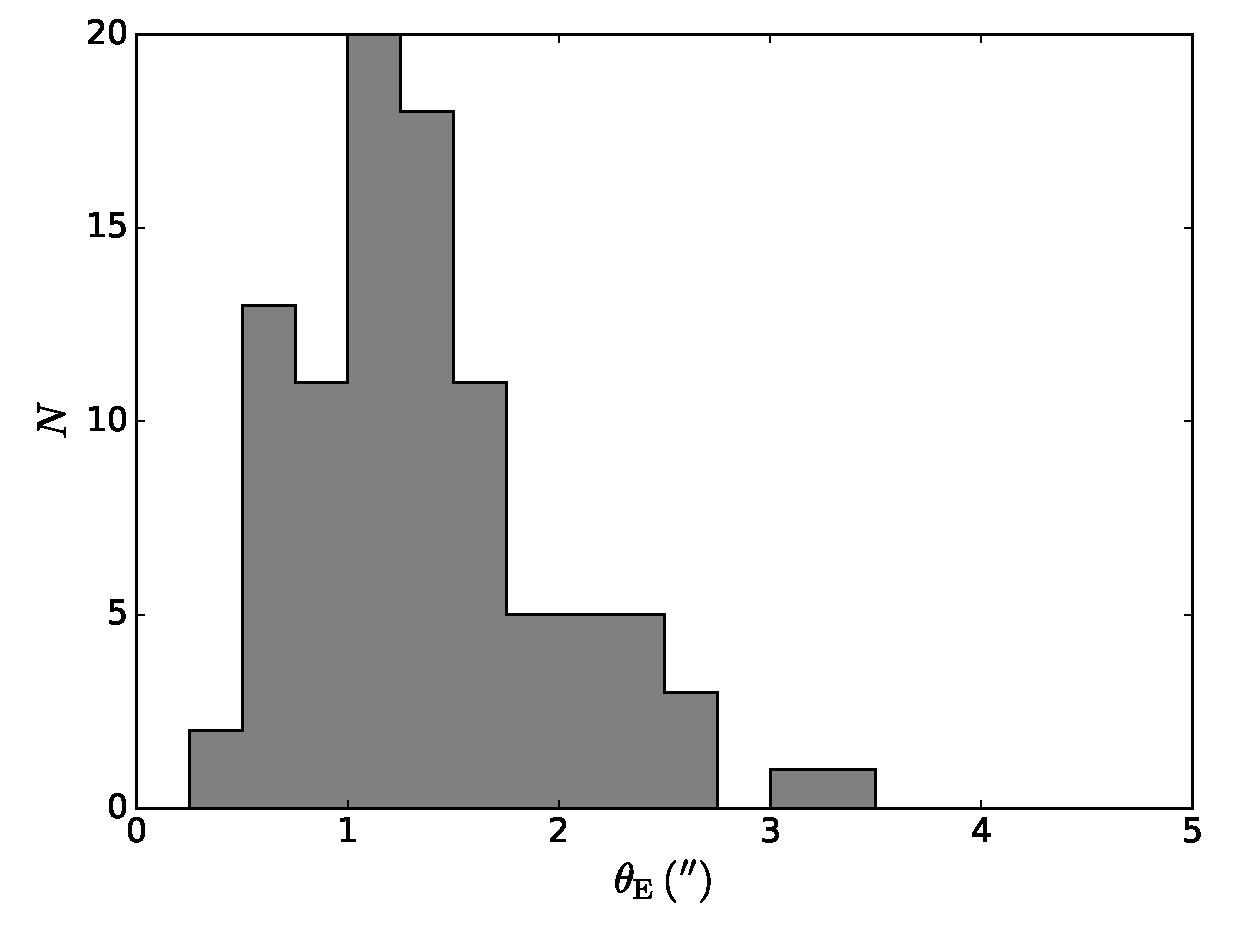
\includegraphics[width=\columnwidth]{rein_hist.eps}
 \caption{Distribution in Einstein radius, in angular units, for the lenses in the mock sample.}
 \label{fig:rein}
\end{figure}
%
%
\begin{figure}
 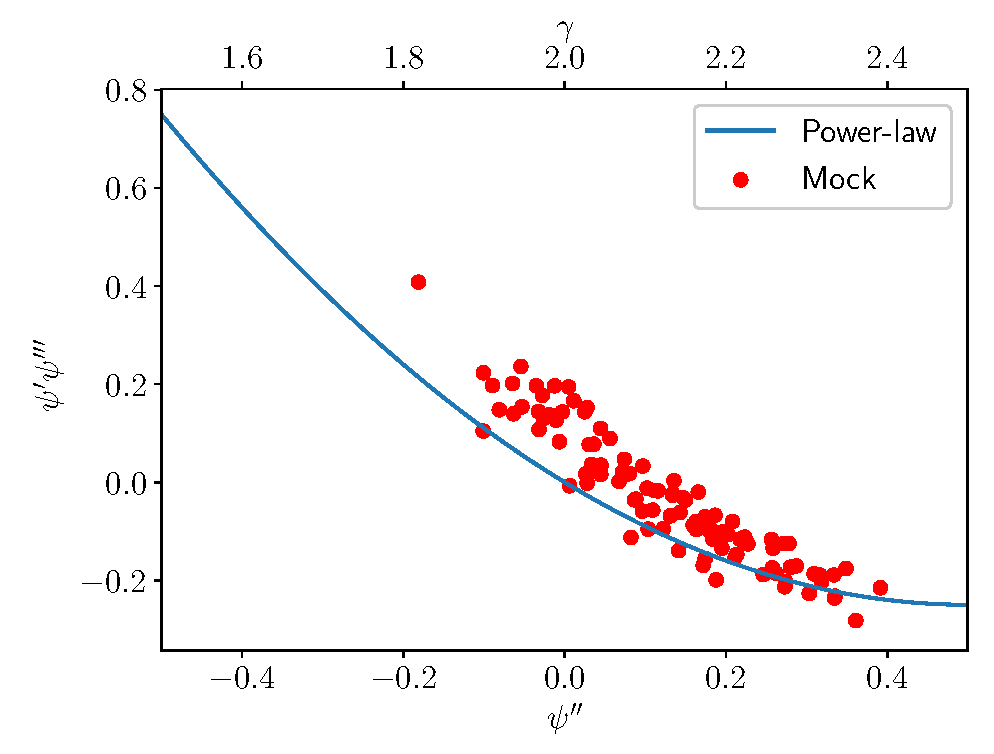
\includegraphics[width=\columnwidth]{psi_plot.eps}
 \caption{Distribution in $\psiii$ and $\psii\psiiii$, respectively the second derivative of the lens potential at the Einstein radius, and the product between the first and third derivative, for the lenses in the mock sample.
The solid line shows the relation between $\psiii$ and $\psii\psiiii$ for a power-law density profile. The top x-axis indicates the value of the power-law slope corresponding to a given value of the second derivative.
}
 \label{fig:psi}
\end{figure}
%
The distribution of lens potential derivatives of our mock galaxies is different from that of a strict power-law profile, though roughly following it.
The farther a lens is from the power-law line in \Fref{fig:psi}, the larger we expect the bias on the time delay cosmology inference introduced by a power-law assumption to be, with the exact value depending on the image configuration of the system.

We then generate mock observations. We add a 0.01~arcsec noise to the image positions, and assume that the radial maagnification ratio between image A and B, $\radmagrat$, is measured with a precision of 0.02.
%Finally, we add a 1~day uncertainty to the time delays.
No uncertainty is added to the time delay at this stage, as our goal is to asses the systematics connected with the lensing analysis alone.

To estimate the amplitude of the bias introduced by a power-law assumption on our mock sample, we simulate a statistical measurement of the cosmological parameter $H_0$.
For simplicity, we focus on the Hubble constant, leaving all other cosmological parameters fixed.

\subsection{Power-law model fits}

For each lens, we fit a power-law density profile to its observed image positions and image magnification ratios. This step is intended to provide similar constraints on the lens density profile as those obtained by detailed modeling of the surface brightness profile of the quasar host galaxy in real lenses.
We assume a flat prior on the Einstein radius, the density slope $\gamma$, and the square of the source distance from the center.
The values of the inferred density slope are plotted in \Fref{fig:slope}, as a function of $2-\psiii$, where $\psiii$ is the true value of the second derivative of the lens potential at the Einstein radius. For a pure power-law profile, $\gamma = 2-\psiii$ (see \Eref{eq:psiiipl}). Therefore, deviations from the 1-1 line in \Fref{fig:slope} indicate deviations from a pure power-law.
%
\begin{figure}
 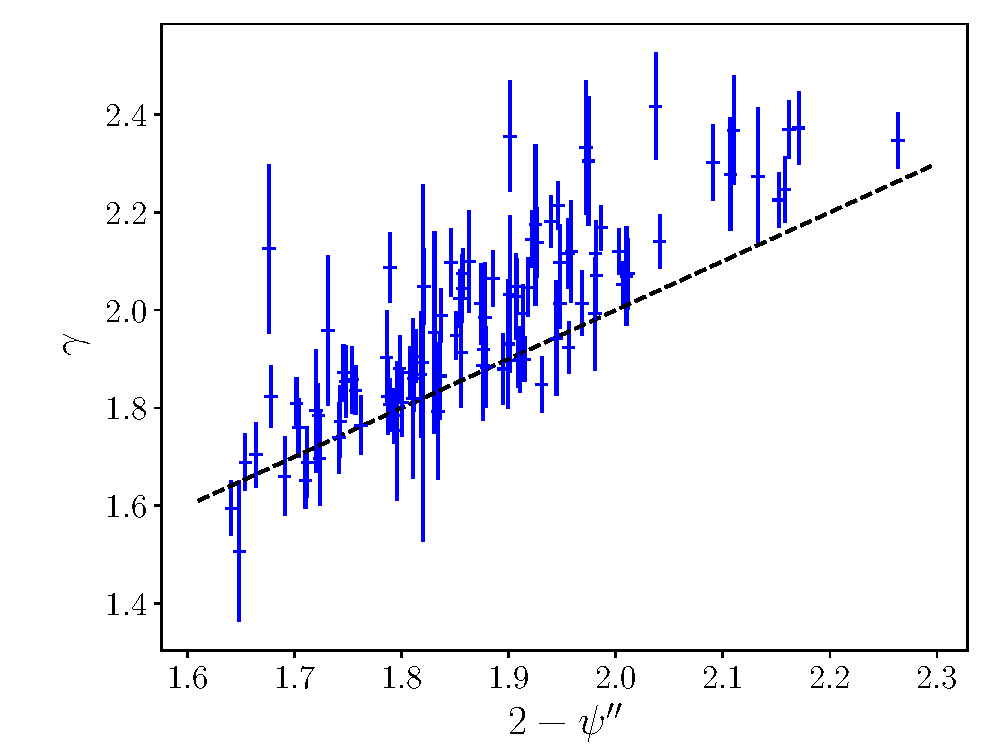
\includegraphics[width=\columnwidth]{gamma_fit.eps}
 \caption{
Inferred values of the density slope $\gamma$, obtained by fitting a power-law density profile to image positions and radial magnification ratios of each mock lens. The values of $\gamma$ are plotted as a function of $2-\psiii$. For a pure power-law density profile we have $\gamma = 2-\psiii$: deviations from the equality line indicate deviations from a pure power-law profile.
Error bars on $\gamma$ indicate the 68\% enclosed probability interval.
}
 \label{fig:slope}
\end{figure}
%
Most data points lie above of the equality line in \Fref{fig:slope}, meaning that the assumption of a power-law density profile underestimates the value of the second derivative (overestimates the quantity $2-\psiii$). This could be inferred by looking at \Fref{fig:psi} as well.

As argued in \Sref{sect:pl}, power-law lenses cannot provide an accurate estimate of the second derivative of the potential, when fitted to image position and radial magnification ratio data.
Image position and radial magnification observations provide information on the following combination of derivatives, instead:
\begin{equation}\label{eq:psicomb}
\psicomb \equiv \frac{\psiiii}{1 - \psiii},
\end{equation}
as can be seen by examining \Eref{eq:imsep} and \Eref{eq:radmagrat}.
We then expect the quantity $\psicomb$ to be recovered relatively well even with power-law models. Let us verify this prediction by plotting the inferred value of $\psicomb$ versus the true values, in \Fref{fig:psicomb}.
%
\begin{figure}
 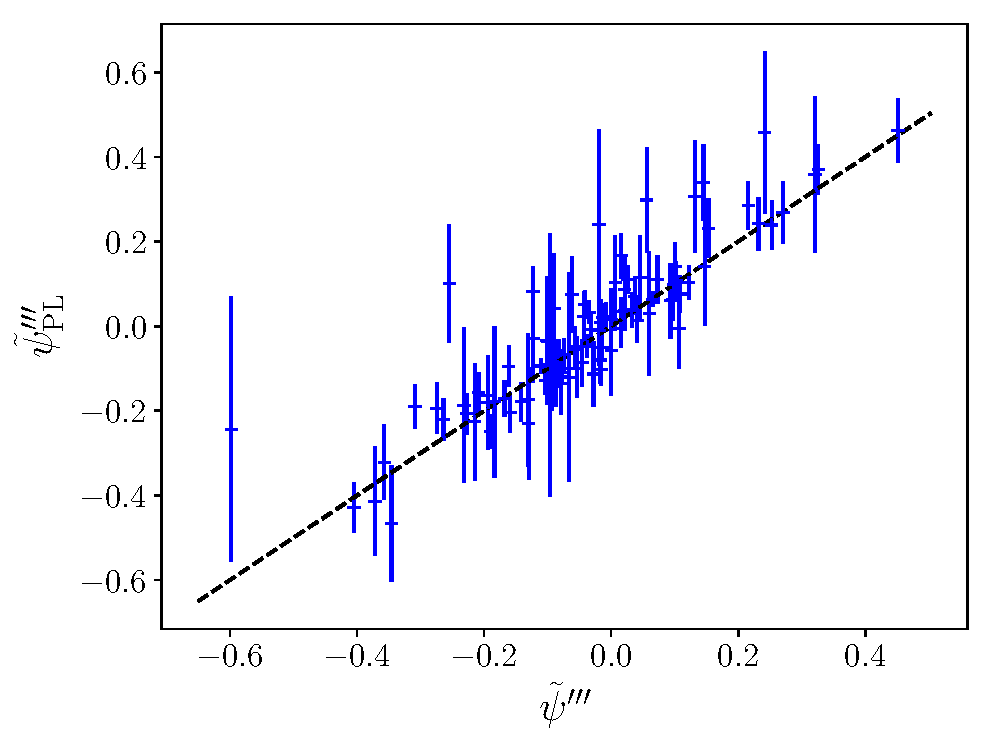
\includegraphics[width=\columnwidth]{psicomb.eps}
 \caption{
Inferred values of the density slope $\gamma$, obtained by fitting a power-law density profile to image positions and radial magnification ratios of each mock lens. The values of $\gamma$ are plotted as a function of $2-\psiii$. For a pure power-law density profile we have $\gamma = 2-\psiii$: deviations from the equality line indicate deviations from a pure power-law profile.
Error bars on $\gamma$ indicate the 68\% enclosed probability interval.
}
 \label{fig:psicomb}
\end{figure}
%
As expected, there is a good match between the true and recovered values.

Let us now comment on the precision on the determination of the slope.
This is essentially set by the uncertainty on the radial magnification ratio and the asymmetry of the image configuration. For image positions close to symmetric, the model magnification ratio is close to unity for a broad range of values of $\gamma$, since the two images probe regions of the potential close to each other, therefore the density slope is largely unconstrained. The impact of changing the density slope on $\radmagrat$ increases for more asymmetric configurations.
For the lenses with the most asymmetric configuration in our mock, the precision on $\gamma$ is $\sim0.04$, which is similar to typical constraints in time delay cosmography studies \citep[see e.g.]{Suy++13}.

\subsection{Inferences on $H_0$}
We now turn our attention to the inference on the Hubble constant.
For each lens, for each value of the model parameters, we then evaluate the model time delay as a function of $H_0$, $\Delta t(H_0)$, using \Eref{eq:dt}:
\begin{multline}
\Delta t (H_0, \gamma, \tein, \beta_s) = \frac{\tilde{H_0}}{H_0}\frac{D_{\Delta t}(\tilde{H_0})}{c} \times \\
\left[\frac{(\theta_A - \beta_s)^2}{2} - \psi(\theta_A) - \frac{(\theta_B - \beta_s)^2}{2} + \psi(\theta_B)\right],
\end{multline}
where $\tilde{H_0}$ is a fiducial value of the Hubble constant, $D_{\Delta t}(\tilde{H_0})$ the time delay distance calculated for $H_0=\tilde{H_0}$, and the image positions and lens potential are a function of the lens model parameters $\gamma$, $\tein$ and $\beta_s$.

By comparing the model time delay with the observed value, and assuming a flat prior on $H_0$, we obtain for each lens the posterior probability distribution of the lens model parameter and the Hubble constant given the data $\data$:
\begin{equation}
\pr(\gamma, \tein, \beta_s, H_0 | \data) = \pr(\gamma, \tein, \beta_s, H_0) \pr(\data | \gamma, \tein, \beta_s, H_0).
\end{equation}
The first term on the right-hand side of the above equation is the prior on the model parameters, while the second term is the likelihood of observing the data given the model.
Since the Hubble constant does not enter the prediction on the image positions and radial magnification ratio, this can be separated as follows:
\begin{multline}
\pr(\data | \gamma, \tein, \beta_s, H_0) = \pr(\theta_{A,B}^{\mathrm{(obs)}},\radmagrat^{\mathrm{(obs)}} | \gamma, \tein, \beta_s) \times \\
\pr(\Delta t^{\mathrm{(obs)}} | \gamma, \tein, \beta_s, H_0).
\end{multline}

We can consider each lens independently, and marginalize over the lens model parameters to obtain a posterior probability distribution on the Hubble constant:
\begin{equation}
\pr(H_0 | \data) = \int d\gamma d\tein d\beta_s \pr(\data | \gamma, \tein, \beta_s, H_0).
\end{equation}
The resulting inference on $H_0$ obtained from each lens is plotted in \Fref{fig:plH0}.
We plot the inferred values of $H_0$ as a function of the following parameter:
\begin{equation}\label{eq:xidef}
\xi \equiv \psiii - \psi''_{\mathrm{PL}}(\psii, \psiiii),
\end{equation}
where $\psi''_{\mathrm{PL}}(\psii, \psiiii)$ is the relation between the second and third derivative of the potential for a power-law lens, given by \Eref{eq:psiiipl_given_psiiii}.
In other words, $\xi$ quantifies the deviation of the true lens density profile from that of a power-law.
We expect the bias on $H_0$ to correlate with $\xi$: since the time delay is, to lowest order in image displacement from the Einstein radius, sensitive to the second derivative of the potential, lenses for which the power-law assumption leads to a wrong inference of $\psiii$ will be the ones with the largest bias.
%
%Since we are mostly concerned with accuracy, we obtained the data points in \Fref{fig:plH0} assuming that the time delay is known exactly, as using realistic errors on $\Delta t$ produces error bars too large to draw any conclusions. The realistic case will be examined later.
%
\begin{figure}
 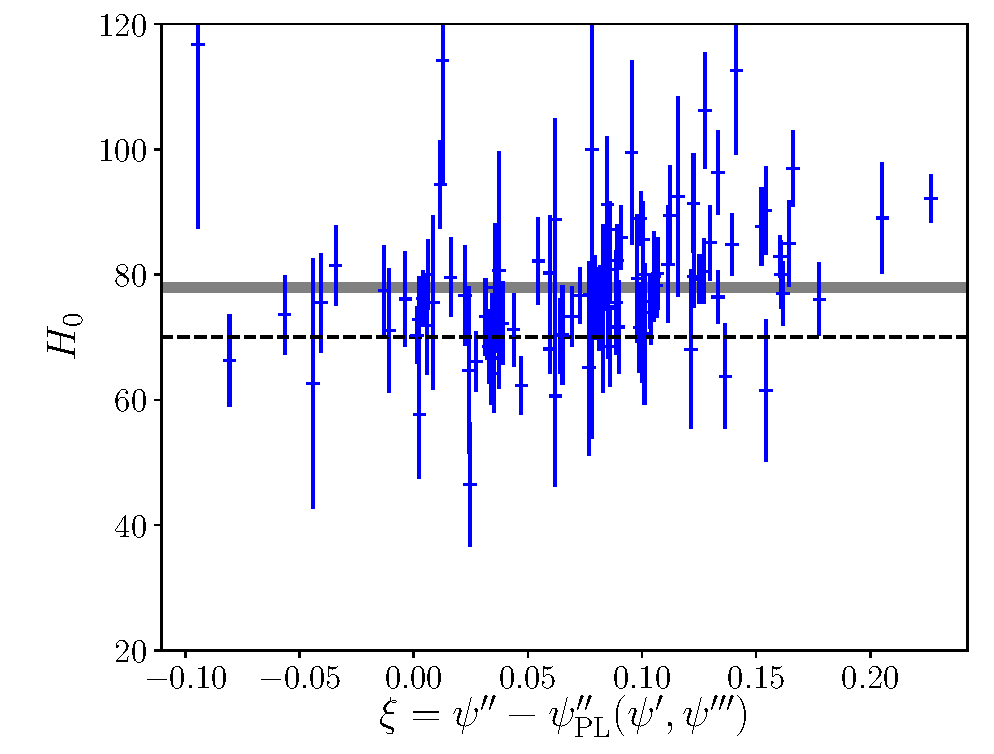
\includegraphics[width=\columnwidth]{individual_H0.eps}
 \caption{Inference on $H_0$ for each lens, obtained by fitting a power-law model to image position and radial magnification data, and to time delay measurements with no uncertainty.
The quantity on the $x$ axis is parameter $\xi$ defined in \Eref{eq:xidef}, quantifying the deviation of the true density profile from that of a power-law.
The dashed horizontal line marks the true value of $H_0$ used to create the mock ($70\,\rm{km}\,\rm{s}^{-1}\,\rm{Mpc}^{-1}$).
The gray horizontal band shows the weighted mean inference on $H_0$, with its 68\% uncertainty region.
}
 \label{fig:plH0}
\end{figure}
%
As expected, we can see a trend between $\xi$ and the inferred value of $H_0$, though with a relatively large scatter.
We then take the weighted mean of the individual measurements, to obtain an ensemble measurement of $H_0$. We use the inverse square errors on the individual $H_0$ measurements as weights.
The result is plotted in \Fref{fig:plH0}. The inference is biased towards larger values by about 10\%.

\section{Flexible models}\label{sect:gnfw}

Power-law models, fitted to image position and radial magnification ratios, cannot provide an accurate estimate of the time-delay of the lenses in our mock sample.
In order to gain in accuracy, we need to increase the flexibility of the model used in the fit, adding at least one degree of freedom to the radial density profile, so that the relation between the second and third derivative of the potential is no longer fixed.

We consider a composite model, with a de Vaucouleurs profile describing the stellar component and a generalized NFW profile (gNFW) to describe the dark matter halo \citep{Zha96}.
\begin{equation}
\rho_{\mathrm{gNFW}}(r) = \frac{\rho_0}{(r/r_s)^\gammadm (1 + r/r_s)^{3 - \beta}}.
\end{equation}
The density profile of a gNFW profile has an inner slope of $\gammadm$ and falls off as $r^{-3}$ at large radii. It reduces to a pure NFW profile for $\gammadm=1$.

We assume that the effective radius of the de Vaucouleurs profile is known exactly.
This assumption leaves one degree of freedom for the stellar component: its total mass.
The dark matter component has three free parameters: mass, inner slope $\gammadm$, and scale radius $r_s$.
We wish to work with a family of models with only three degrees of freedom in total.
Therefore, we arbitrarily fix the scale radius of the halo to ten times the effective radius:
\begin{equation}\label{eq:scaleradius}
r_s = 10 \reff.
\end{equation}
%The free parameters of the model then are: stellar mass $M_*$, dark matter inner slope $\beta$, and a normalization for the dark matter halo. Since 
Due to this choice, our model cannot provide a perfect description of the galaxies in our mock: although mock halos have an NFW density profile, their scale radius is assigned through a mass-concentration relation with scatter. Therefore they do not satisfy \Eref{eq:scaleradius}.
Nevertheless, as we will show, this model can still allow us to make an accurate prediction on the time delay, thanks to its flexibility.
%We do not expect this to be a problem in terms of accuracy on the time delay: our analysis in \Sref{sect:pot} guarantees that an accurate estimate of $\Delta t$ can be obtained 

We have increased the number of degrees of freedom in the radial density profile from two to three.
Obviously, this new model cannot be fully constrained with only two image positions and one measurement of the radial magnfication ratio.
In order to make an inference on the time delay, additional constraints are needed.
We consider the central velocity dispersion as a new observable.
Velocity dispersion information is often used in time delay cosmology measurements to improve the precision and accuracy of the model \citep{Suy++14,Won++17}.

For each mock lens, we use the spherical Jeans equation to calculate its surface brightness-weighted line-of-sight velocity dispersion, integrated within a circular aperture of radius $\reff/2$, which we denote $\sigmae$. We assume isotropic orbits. Then, we add a Gaussian noise with a $10\,\rm{km}\,{s}^{-1}$ scatter. We do not convolve the velocity dispersion by an artificial point spread function, for the sake of saving computational time.

We fit our composite model to image position, radial magnification ratio and velocity dispersion of each mock lens. For a given set of parameter values, we calculate a model velocity dispersion in the same way we generated the data, by using the spherical Jeans equation under the assumption of isotropic orbits. Essentially, we are assuming that the line-of-sight structure and orbital anisotropy profile of the lens is known exactly, which is a very optimistic assumption.

We parametrize the normalization of the dark matter halo in terms of the projected mass enclosed within $\reff$, labeled $\mdme$.
We assume flat priors on $\log{M_*}$, $\log{\mdme}$, $\gammadm$ and the square of the source position.
We first fit the model to lensing constraints only. The inference is plotted in \Fref{fig:onelens} (solid lines). As expected, image positions and radial magnification ratio alone cannot constrain the model, and the inference is largely driven by the prior.
When velocity dispersion information is included, the model converges to a well defined solution (red contours in \Fref{fig:onelens}).
%In \Fref{fig:onelens}, we show the inference on the model parameters for one lens in the mock sample (red contours). 
In addition to the four parameter listed above, we also show the inference on the different derivatives of the lens potential, as well as the time delay.
Significantly, the addition of velocity dispersion information helps narrow down the uncertainty on the second derivative of the lensing potential.
As a result, the predicted time delay is accurate.
%
\begin{figure*}
 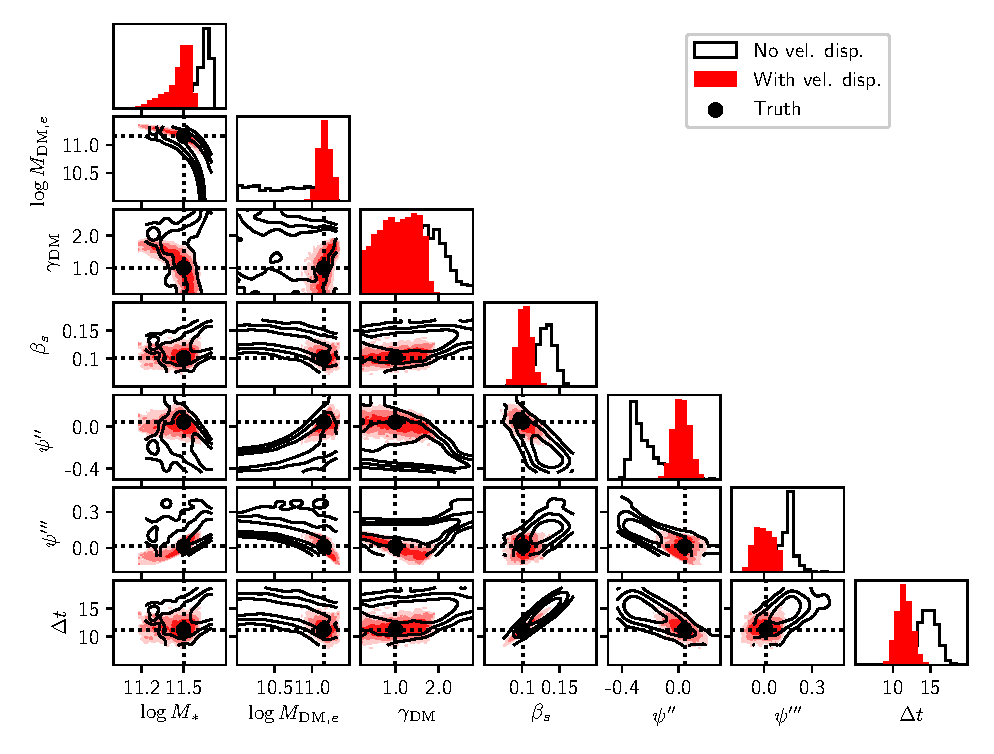
\includegraphics[width=\textwidth]{gnfw_cornerplot.eps}
 \caption{
{\em Solid lines:} posterior probability distribution on the model parameters obtained by fitting a composite de Vaucouleurs + gNFW model to image position and radial magnification ratio of a mock lens.
{\em Red contours:} inference obtained by adding velocity dispersion information.
Different contour levels indicate the 68\%, 95\% and 99.7\% enclosed probability regions.
The black dots indicate the true values.
In addition to the free parameters of the model (stellar mass $M_*$, projected dark matter enclosed within the effective radius $\mdme$, inner dark matter slope $\gammadm$ and source position $\beta_s$), we show the inference on the second and third derivatives of the lens potential at the Einstein radius, as well as the time delay between the two images.
}
 \label{fig:onelens}
\end{figure*}
%

We fit all 100 lenses in the mock, then, similarly to \Sref{sect:pl}, we obtain an inference on $H_0$ for each lens.
However, unlike in \Sref{sect:pl}, we add a 1 day observational uncertainty to the time delay.
While the goal of the previous fit was to show that power-law models give a biased answer, here we wish to show that we can recover the truth even in case of observational errors.
Adding noise to the time delay not only increases the error bar on individual measurements, but it also shifts the weight towards systems with larger image asymmetry, for which the time delay is larger and, therefore, more easily measurable.
Increasing the weight for systems with large asymmetry can in principle bias the result, because, as \Eref{eq:dt2nd} shows, going to larger values of $\Delta\theta_A$ requires a more accurate knowledge of higher derivatives of the potential in order to make accurate time delay predictions.

Individual $H_0$ measurements and the weighted mean measurement over the whole sample are plotted in \Fref{fig:gnfw_indH0}.
The Hubble constant is recovered at better than 1\% accuracy.
%
\begin{figure}
 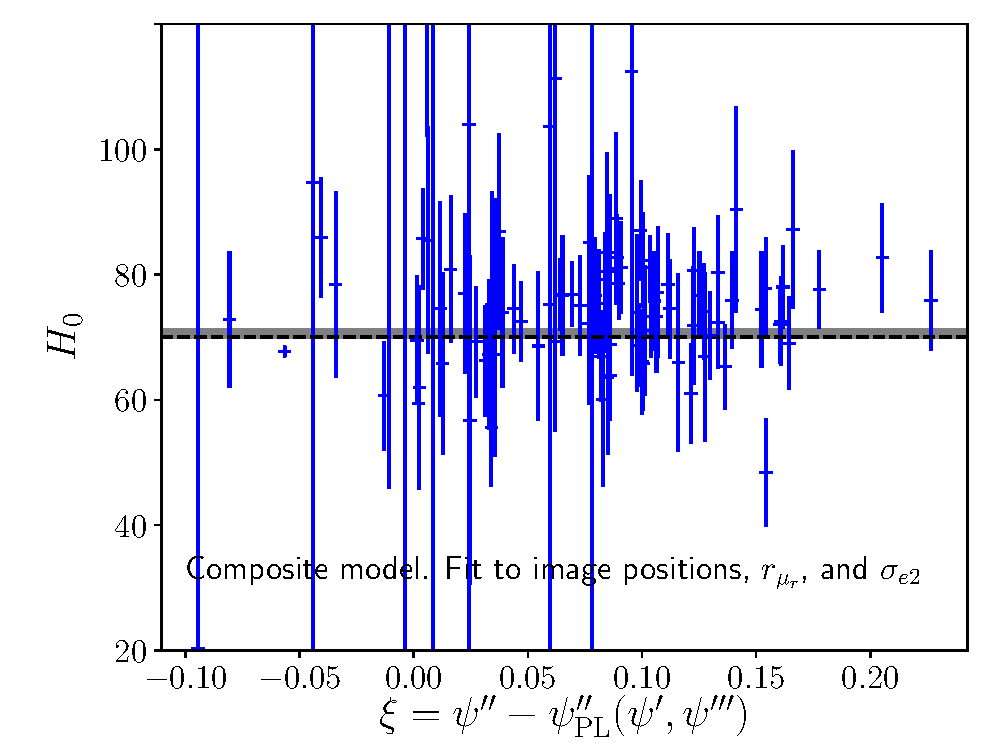
\includegraphics[width=\columnwidth]{gnfw_individual_H0.eps}
 \caption{Inference on $H_0$ for each lens, obtained by fitting a composite de Vaueouleurs + gNFW model to image position, radial magnification ratio, velocity dispersion, and to time delay measurements with 1 day uncertainty.
The quantity on the $x$ axis is parameter $\xi$ defined in \Eref{eq:xidef}, quantifying the deviation of the true density profile from that of a power-law.
The dashed horizontal line marks the true value of $H_0$ used to create the mock ($70\,\rm{km}\,\rm{s}^{-1}\,\rm{Mpc}^{-1}$).
The gray horizontal band shows the weighted mean inference on $H_0$, with its 68\% uncertainty region.
}
 \label{fig:gnfw_indH0}
\end{figure}
%

The excellent agreement between the value of $H_0$ obtained with our flexible model thanks to the addition of velocity dispersion information raises a question: would it be possible to make a similarly accurate inference using power-law profiles, if we replace the radial magnification constraint with the velocity dispersion?
As pointed out eariler, the radial magnification ratio is mostly sensitive to the third derivative of the potential. Although this piece of information can be use to get a high precision measurement of the power-law slope $\gamma$, it does not help in the prediction of the time delay, since an accurate knowledge of $\psiii$ is required to constrain the latter.

We then revert to power-law models and fit them to image position and velocity dispersion data only.
The individual inferences on $H_0$ and the ensemble measurement are plotted in \Fref{fig:pl_indH0_wdyn}.
The population average Hubble constant is now only 2\% larger than the truth, a remarkable improvement compared to the 10\% bias obtained in \Sref{sect:pl} with purely lensing constraints.
%
\begin{figure}
 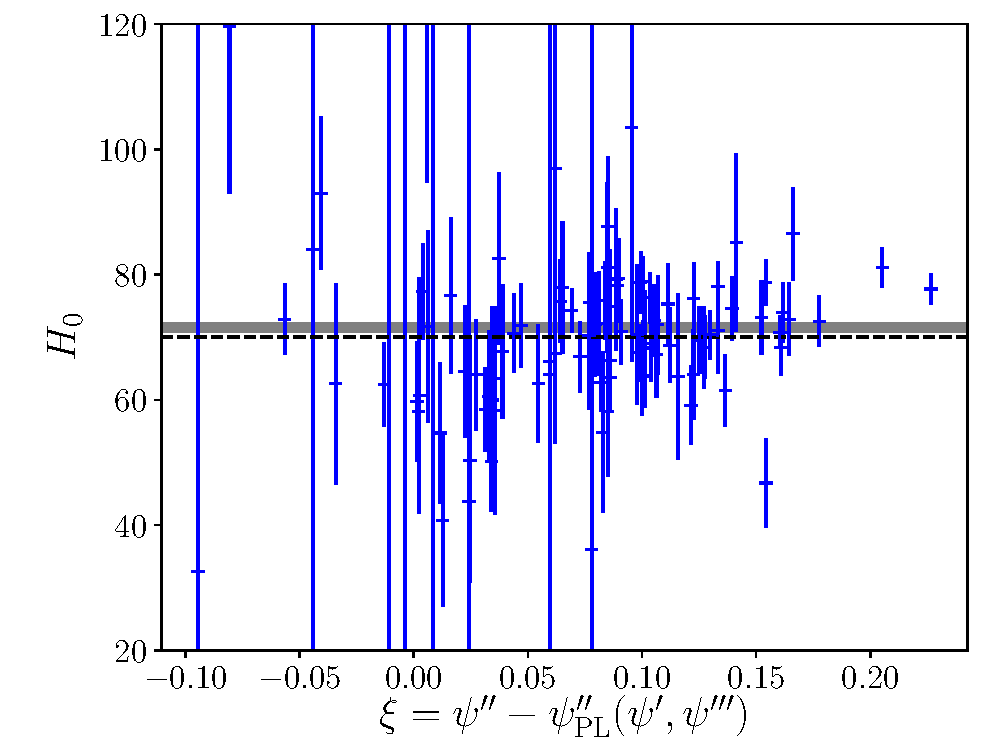
\includegraphics[width=\columnwidth]{pl_impos_dyn_individual_H0.eps}
 \caption{Inference on $H_0$ for each lens, obtained by fitting a power-law model to image position, velocity dispersion, and to time delay measurements with one day uncertainty.
The quantity on the $x$ axis is parameter $\xi$ defined in \Eref{eq:xidef}, quantifying the deviation of the true density profile from that of a power-law.
The dashed horizontal line marks the true value of $H_0$ used to create the mock ($70\,\rm{km}\,\rm{s}^{-1}\,\rm{Mpc}^{-1}$).
The gray horizontal band shows the weighted mean inference on $H_0$, with its 68\% uncertainty region.
}
 \label{fig:pl_indH0_wdyn}
\end{figure}
%
\section{Discussion}

On the basis of simple analytical arguments, we predicted in \Sref{sect:pot} that, in order to model time delays with an accuracy of a few percent, a class of lens models with at least three degrees of freedom in the radial profile is needed.
This conclusion cast doubts on the adequacy of power-law models in time delay cosmography studies.
Indeed, tests performed on mock lensing observations showed that using power-law models can lead to a 10\% bias on the inference of the Hubble constant.
However, this finding is in apparent contradiction with the last result shown in \Sref{sect:gnfw}: fitting the same power-law models to the quasar image position and velocity dispersion data, and ignoring magnification information, gives a much more accurate answer.

The problem does not lie with power-law models themselves, but rather with the data used to constrain their parameters.
In detailed lensing studies, the slope of the lens density profile is typically measured by fitting a power-law model to the surface brightness distribution of the arcs.
However, as we argued in \Sref{sect:pot}, this is only a measurement of radial magnification ratio, which to first nontrivial order is mostly sensitive to the third derivative of the potential.
The second derivative of the potential, more important for the determination of the time delay, is then assigned by a fixed relation, \Eref{eq:psiiipl_given_psiiii}, introducing a bias.

A possible alternative, or complementary information, to radial magnification ratios, is the use of stellar kinematics.
However, relying on velocity dispersion information to accurately constrain lens models is a difficult taks.
Although our tests performed in \Sref{sect:gnfw} showed promising results, they were based on a set of optimistic assumptions: in particular, spherical symmetry and isotropic orbits.
In real applications, projection effects and orbital anisotropy can introduce large biases if not carefully accounted for.
Spatially resolved kinematic information, such as velocity measurements from integral field spectroscopy, is most likely necessary for an accuracy goal of a few percent.

Our analytical treatment of \Sref{sect:pot}, as well as all of our tests, is based on a strong assumption: that of circular symmetry.
Axisymmetric lenses are qualitatively different from more realistic models.
For instance, their critical curves, isopotential and isodensity contours have all the same shape.
This is not true in general, and, as a result, the equations derived in \Sref{sect:pot} are not strictly applicable to most lenses.

One consequence of the departure from circular symmetry is that, for doubles, as the source crosses the tangential caustic, only one of the two images touches the critical curve.
In other words, as $\Delta\theta_A$, interpreted as distance from the tangential critical curve in an appropriate coordinate frame, goes to zero, $\Delta\theta_B$ approaches a finite value.
Nevertheless, for moderate ellipticities, our main results are still qualitatively correct.
The time delay is still proportional, to leading order in image displacement from the critical curve, to the difference in deflection angles at the location of the two images.
This introduces a dependence on the second derivative of the potential.

The radial magnification ratio is, to first nontrivial order in image position, a difference in the radial eigenvalue of the lens Jacobian matrix, which introduces a dependence on the third derivative of the potential.
Therefore, we expect, even in the general case, that radial magnification ratio information alone would not be sufficient to make an accurate time delay prediction.

Another consequence of the assumption of spherical symmetry is 
 the relatively large number of doubles with image positions close to the critical curve compared to real samples.
Adding a realistic distribution in lens flattening would turn many of our mock lenses into four image systems.
This limits somewhat our ability to generalize our results, especially because we limited our analysis to systems with small image asymmetry.
Although in \Sref{sect:gnfw} we showed that a family of models with three parameters can give a very accurate description of the lenses in our mock, the same might not be true for systems with a significantly more asymmetric image configuraton, more typical of doubles, as the radial range over which the potential needs to be accurately characterized becomes larger.

\section{Conclusion}



\section*{acknowledgments}
This work was supported by World Premier International Research Center Initiative (WPI Initiative), MEXT, Japan.
AS is partly supported by KAKENHI Grant Number JP17K14250. 
%-------------------------------------------------------------------------------
\bibliographystyle{mnras}
\bibliography{references}
%-------------------------------------------------------------------------------

\end{document}
%===============================================================================
